\chapter[APÊNDICE \ref{Ap:Shell-cyl}]{Cilindro biengastado em problema estático}
\label{Ap:Shell-cyl}

Outro problema comum considera um cilindro sujeito a duas cargas concentradas diametralmente opostas, conforme visto na Figura \ref{fig:cylinder-shell}. As dimensões do problema são: comprimento $L=600$, raio $R=300$ e espessura $t=3$. A carga aplicada é $P=1$. O material que constitui o cilindro possui módulo de elasticidade $E=3\times10^6$ e coeficiente de Poisson $\nu=0,3$. Ambas as extremidades do cilindro estão vinculadas a um diafragma rígido, ou seja, $u_1=u_3=\phi_2=0$. O resultado de referência adotado é de um deslocamento radial de $1,8248\times10^{-5}$ no ponto de aplicação da carga \cite{BELYTSCHKO1985221,CHAUDINH2023110222,ZHOU2022108568}.

\begin{figure}[h!]
    \centering
    \caption{Cilindro submetido a forças concentradas.}
    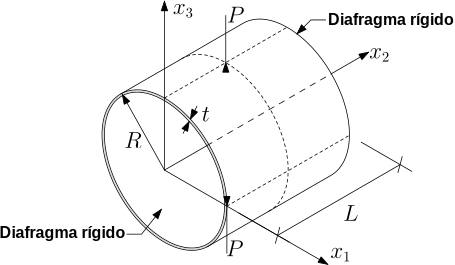
\includegraphics[width=0.65\linewidth]{Figuras/cylinder-shell/cylinder.pdf}
    \\Fonte: Autoria Própria (\the\year).
    \label{fig:cylinder-shell}
\end{figure}

Pelo fato do problema apresentar simetria, foi estudado somente um octante do problema. Assim utilizou-se uma malha não-estruturada, com refinamento maior próximo ao ponto de aplicação da força, contendo 810 elementos triangulares de aproximação quadrática, contando com um total de 11977 graus de liberdade. A malha utilizada é observada na Figura \ref{fig:cylinder-shell-mesh}. Na simulação adotou-se uma única iteração de Newton-Raphson.

\begin{figure}[h!]
    \centering
    \caption{Malha utilizada na simulação de cilindro biengastado.}
    \includegraphics[width=0.3\linewidth]{Figuras/cylinder-shell/mesh1.png}
    \\Fonte: Autoria Própria (\the\year).
    \label{fig:cylinder-shell-mesh}
\end{figure}

O resultado obtido foi de um deslocamento radial de $1,8135\times10^{-5}$, tendo, portanto, um desvio relativo de $0,6176\%$ em relação à referência. Os campos de deslocamentos obtidos são apresentados na Figura \ref{fig:cylinder-shell-disp}, os quais são muito próximos aos obtidos por \citeonline{ZHOU2022108568}.

\begin{figure}[h!]
    \centering
    \caption{Campos de deslocamentos obtido na simulação de cilindro.}
    \begin{subfigure}{0.075\textwidth}
        \includegraphics[width=\linewidth]{Figuras/cylinder-shell/eixos.png}
    \end{subfigure}
    \begin{subfigure}{0.3\textwidth}
        \includegraphics[width=\linewidth]{Figuras/cylinder-shell/ux.png}
    \end{subfigure}
    \begin{subfigure}{0.3\textwidth}
        \includegraphics[width=\linewidth]{Figuras/cylinder-shell/uy.png}
    \end{subfigure}
    \begin{subfigure}{0.3\textwidth}
        \includegraphics[width=\linewidth]{Figuras/cylinder-shell/uz.png}
    \end{subfigure}
    \\Fonte: Autoria Própria (\the\year).
    \label{fig:cylinder-shell-disp}
\end{figure}

Também se comparou o resultado obtido com relação à uma simulação feita no \textit{software} ANSYS, a qual resultou em um deslocamento de $1,8190\times10^{-5}$. Logo o desvio do resultado calculado com o apresentado pelo ANSYS foi de $0,3007\%$. Além disso, verificou-se o deslocamento radial ao longo das arestas compreendidas pela interseção do cilindro com o plano $x_1=0$ e com $x_2=L/2$. A Figura \ref{fig:cylinder-shell-deslradial} ilustra graficamente os resultados obtidos.

\begin{figure}[h!]
    \centering
    \caption{Deslocamentos radiais ao longo da aresta compreendida pela interseção do cilindro como o plano:}
    \begin{subfigure}{0.49\textwidth}
        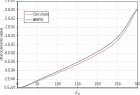
\includegraphics[width=\linewidth]{Figuras/cylinder-shell/deslocamento1.pdf}
        \caption{$x_1=0$}
    \end{subfigure}
    \begin{subfigure}{0.49\textwidth}
        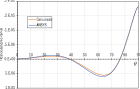
\includegraphics[width=\linewidth]{Figuras/cylinder-shell/deslocamento2.pdf}
        \caption{$x_2=L/2$}
    \end{subfigure}
    \\Fonte: Autoria Própria (\the\year).
    \label{fig:cylinder-shell-deslradial}
\end{figure}